\documentclass[a4paper,11pt,twoside]{memoir}
\chapterstyle{veelo}

\usepackage{TUINFDA}

\usepackage{url}
\usepackage{hyperref}					% links in pdf
\usepackage{graphicx}            			% Figures
\usepackage{verbatim}            			% Code-Environment
\usepackage[lined,linesnumbered,algochapter]{algorithm2e} % Algorithm-Environment

\usepackage{pgf}					
\usepackage{tikz}					% tikz graphics
\usetikzlibrary{arrows,automata}

\usepackage{ngerman}
\usepackage[ngerman]{babel}
\usepackage{bibgerm,cite}       % Deutsche Bezeichnungen, Automatisches Zusammenfassen von Literaturstellen
\usepackage[ngerman]{varioref}  % Querverweise
% to use the german charset include cp850 for MS-DOS, ansinew for Windows and latin1 for Linux.
% \usepackage[latin1]{inputenc}

\thesistitle{Title of the Thesis}
\thesissubtitle{Optional Subtitle} % optional
\thesisdate{TT.MM.JJJJ}

% all titles and designations have to be gender-related!
\thesisdegree{Diplom-Ingenieurin}{Diplom-Ingenieurin}
\thesiscurriculum{Wirtschaftsinformatik}{Business Informatics} % your study
\thesisverfassung{Verfasserin} % Verfasser
\thesisauthor{Martina Musterfrau} % your name
\thesisauthoraddress{Musterplatz 1, 1111 Wien} % your address
\thesismatrikelno{0123456} % your registration number

\thesisbetreins{o.Univ.-Prof. Dipl.-Ing. Mag. Dr. Monika Musterprofessorin}
\thesisbetrzwei{Dr. Vorname Familienname}
\thesisbetrdrei{Dr. Vorname Familienname} % optional

% define page numbering styles
\makepagestyle{numberCorner}
\makeevenfoot{numberCorner}{\thepage}{}{}
\makeoddfoot{numberCorner}{}{}{\thepage}

% define custom macros for specific formats or names
\newcommand{\uml}[1]{\texttt{#1}}
\newcommand{\cd}{\textsf{Class Diagram}}

\begin{document}

\captionnamefont{\bfseries}

%%%%%%%%%%%%%%%%%%%%%%%%%%%%%%%%%%%%%%%%%
%%%   FRONTMATTER    %%%%%%%%%%%%%%%%%%%%
%%%%%%%%%%%%%%%%%%%%%%%%%%%%%%%%%%%%%%%%%
\frontmatter
\pagenumbering{roman}

%%%%%%%%%%%%%%%%%%%%%%%%%%%%%%%%%%%%%%%%%
%%%   TITLEPAGES    %%%%%%%%%%%%%%%%%%%%%
%%%%%%%%%%%%%%%%%%%%%%%%%%%%%%%%%%%%%%%%%

% the german title page is required as first page
% $Id: titlepage.tex 1752 2010-03-20 11:07:02Z tkren $
%
% TU Wien - Faculty of Informatics
% thesis titlepage
%
% This titlepage is using the geometry package, see
% <http://www.ctan.org/macros/latex/contrib/geometry/geometry.pdf>
%
% For questions and comments send an email to
% Thomas Krennwallner <tkren@kr.tuwien.ac.at>
% or to Petra Brosch <brosch@big.tuwien.ac.at>
%

\selectlanguage{ngerman}

% setup page dimensions for titlepage
\newgeometry{left=2.4cm,right=2.4cm,bottom=2.5cm,top=2cm}

% force baselineskip and parindent
\newlength{\tmpbaselineskip}
\setlength{\tmpbaselineskip}{\baselineskip}
\setlength{\baselineskip}{13.6pt}
\newlength{\tmpparindent}
\setlength{\tmpparindent}{\parindent}
\setlength{\parindent}{17pt}

% first titlepage
\thispagestyle{tuinftitlepage}

%
% Kludge: for each titlepage set \pagenumbering to a different
% style. This is used to fix a problem with hyperref, because there
% are multiple "page 1" and hyperref hates that
%
\pagenumbering{Alph}

\begin{center}
{\ \vspace{3.4cm}}

\begin{minipage}[t][2.8cm][s]{\textwidth}%
\centering
\thesistitlefontHUGE\sffamily\bfseries\tuinfthesistitle\\
\bigskip
{\thesistitlefonthuge\sffamily\bfseries\tuinfthesissubtitle}
\end{minipage}

\vspace{1.3cm}

{\thesistitlefontLARGE\sffamily \tuinfthesistype}

\vspace{6mm}

%{\thesistitlefontlarge\sffamily zur Erlangung des akademischen Grades}
%
%\vspace{6mm}
%
%{\thesistitlefontLARGE\sffamily\bfseries \tuinfthesisdegree}
%
%\vspace{6mm}
%
%{\thesistitlefontlarge\sffamily im Rahmen des Studiums}
%
%\vspace{6mm}
%
%{\thesistitlefontLarge\sffamily\bfseries \tuinfthesiscurriculum}
%
%\vspace{6.5mm}

{\thesistitlefontlarge\sffamily von}

\vspace{6mm}

{\thesistitlefontLarge\sffamily\bfseries \tuinfthesisauthor}

\vspace{1.5mm}

{\thesistitlefontlarge\sffamily Matrikelnummer \tuinfthesismatrikelno} 

\vspace{3cm} %default: 1.4cm



\begin{minipage}[t][4cm][t]{\textwidth}%
  \vspace{0pt}\raggedright\thesistitlefontnormalsize\sffamily
  %
  \centering
  
  unter der Betreuung von 
  
  \tuinfthesisbetreins
  
%  \begin{tabbing}%
%	    \hspace{19mm} \= \hspace{66mm} \kill
%	    betreut von \> \tuinfthesisbetreins\\
%%	    Mitwirkung: \> \tuinfthesisbetrzwei\\
%%	                \> \tuinfthesisbetrdrei
%  \end{tabbing}
\end{minipage}

\vspace{0pt}\raggedright\thesistitlefontnormalsize\sffamily
\begin{minipage}[t][1.6cm][t]{\textwidth}%
  %
  \centering

  Interactive Media Systems Group

  Institut f\"ur Softwaretechnik und Interaktive Systeme

  Fakult\"{a}t f\"{u}r Informatik 

  Technische Universit\"{a}t Wien

\end{minipage}



%\begin{minipage}[t][1.5cm][t]{\textwidth}%
%  \vspace{0pt}\sffamily\thesistitlefontnormalsize
%  \begin{tabbing}%
%    \hspace{45mm} \= \hspace{63mm} \= \hspace{51mm} \kill
%    Wien, \tuinfthesisdate \> {\raggedright\rule{51mm}{0.5pt}} \> {\raggedright\rule{51mm}{0.5pt}} \\
%    \> \begin{minipage}[t][0.5cm][t]{51mm}\centering (Unterschrift \tuinfthesisverfassung)\end{minipage}
%    \> \begin{minipage}[t][0.5cm][t]{51mm}\centering (Unterschrift \tuinfthesisbetreuung)\end{minipage}
%    \end{tabbing}
%\end{minipage}

\end{center}

% we want an empty page right after first titlepage
\pagestyle{empty}
\cleardoublepage

% we're done with the titlepages, proceed with default pagenumbering
\pagenumbering{roman}

% restore baselineskip
\setlength{\baselineskip}{\tmpbaselineskip}
\setlength{\parindent}{\tmpparindent}

% back to normal geometry
\restoregeometry

\selectlanguage{english}

%%% Local Variables:
%%% TeX-PDF-mode: t
%%% TeX-debug-bad-boxes: t
%%% TeX-parse-self: t
%%% TeX-auto-save: t
%%% reftex-plug-into-AUCTeX: t
%%% End:


% an english translation may follow
% $Id: titlepage.tex 1752 2010-03-20 11:07:02Z tkren $
%
% TU Wien - Faculty of Informatics
% thesis titlepage
%
% This titlepage is using the geometry package, see
% <http://www.ctan.org/macros/latex/contrib/geometry/geometry.pdf>
%
% For questions and comments send an email to
% Thomas Krennwallner <tkren@kr.tuwien.ac.at>
% or to Petra Brosch <brosch@big.tuwien.ac.at>
%

% setup page dimensions for titlepage
\newgeometry{left=2.4cm,right=2.4cm,bottom=2.5cm,top=2cm}

% force baselineskip and parindent
%\newlength{\tmpbaselineskip}
%\setlength{\tmpbaselineskip}{\baselineskip}
%\setlength{\baselineskip}{13.6pt}
%\newlength{\tmpparindent}
%\setlength{\tmpparindent}{\parindent}
%\setlength{\parindent}{17pt}

% first titlepage
\thispagestyle{tuinftitlepage}

%
% Kludge: for each titlepage set \pagenumbering to a different
% style. This is used to fix a problem with hyperref, because there
% are multiple "page 1" and hyperref hates that
%
\pagenumbering{Roman}

\begin{center}
{\ \vspace{3.4cm}}

\begin{minipage}[t][2.8cm][s]{\textwidth}%
\centering
\thesistitlefontHUGE\sffamily\bfseries\tuinfthesistitle\\
\bigskip
{\thesistitlefonthuge\sffamily\bfseries\tuinfthesissubtitle}
\end{minipage}

\vspace{1.3cm}

{\thesistitlefontLARGE\sffamily \tuinfthesistypeen}

\vspace{6mm}

{\thesistitlefontlarge\sffamily submitted in partial fulfillment of the requirements for the degree of}

\vspace{6mm}

{\thesistitlefontLARGE\sffamily\bfseries \tuinfthesisdegreeen}

\vspace{6mm}

{\thesistitlefontlarge\sffamily in}

\vspace{6mm}

{\thesistitlefontLarge\sffamily\bfseries \tuinfthesiscurriculumen}

\vspace{6.5mm}

{\thesistitlefontlarge\sffamily by}

\vspace{6mm}

{\thesistitlefontLarge\sffamily\bfseries \tuinfthesisauthor}

\vspace{1.5mm}

{\thesistitlefontlarge\sffamily Registration Number \tuinfthesismatrikelno} 

\vspace{1.4cm}

\begin{minipage}[t][1.6cm][t]{\textwidth}%
  \vspace{0pt}\raggedright\thesistitlefontnormalsize\sffamily
  %
  to the Faculty of Informatics 

  at the Vienna University of Technology
\end{minipage}

\vspace{0pt}\raggedright\thesistitlefontnormalsize\sffamily
\begin{minipage}[t][4cm][t]{\textwidth}%
  \begin{tabbing}%
	    \hspace{19mm} \= \hspace{66mm} \kill
	    Advisor: \> \tuinfthesisbetreins\\
	    Assistance: \> \tuinfthesisbetrzwei\\
	                \> \tuinfthesisbetrdrei
     \end{tabbing}
\end{minipage}

\begin{minipage}[t][1.5cm][t]{\textwidth}%
  \vspace{0pt}\sffamily\thesistitlefontnormalsize
  \begin{tabbing}%
    \hspace{45mm} \= \hspace{63mm} \= \hspace{51mm} \kill
    Vienna, \tuinfthesisdate \> {\raggedright\rule{51mm}{0.5pt}} \> {\raggedright\rule{51mm}{0.5pt}} \\
    \> \begin{minipage}[t][0.5cm][t]{51mm}\centering (Signature of Author)\end{minipage}
    \> \begin{minipage}[t][0.5cm][t]{51mm}\centering (Signature of Advisor)\end{minipage}
    \end{tabbing}
\end{minipage}

\end{center}

% we want an empty page right after first titlepage
\pagestyle{empty}
\cleardoublepage

% we're done with the titlepages, proceed with default pagenumbering
\pagenumbering{roman}

% restore baselineskip
\setlength{\baselineskip}{\tmpbaselineskip}
\setlength{\parindent}{\tmpparindent}

% back to normal geometry
\restoregeometry


%%% Local Variables:
%%% TeX-PDF-mode: t
%%% TeX-debug-bad-boxes: t
%%% TeX-parse-self: t
%%% TeX-auto-save: t
%%% reftex-plug-into-AUCTeX: t
%%% End:
 % optional

%%%%%%%%%%%%%%%%%%%%%%%%%%%%%%%%%%%%%%%%%
%%%   ERKLAERUNG DER SELBSTAENDIGKEIT   %
%%%%%%%%%%%%%%%%%%%%%%%%%%%%%%%%%%%%%%%%%
\cleardoublepage
\selectlanguage{ngerman}
\chapter*{Erklärung zur Verfassung der Arbeit}

\tuinfthesisauthor\\
\tuinfthesisauthoraddress

\vspace*{1.2cm}

Hiermit erkläre ich, dass ich diese Arbeit selbständig verfasst habe, 
dass ich die verwendeten Quellen und Hilfsmittel vollständig angegeben 
habe und dass ich die Stellen der Arbeit - einschließlich Tabellen, 
Karten und Abbildungen -, die anderen Werken oder dem Internet im 
Wortlaut oder dem Sinn nach entnommen sind, auf jeden Fall unter Angabe 
der Quelle als Entlehnung kenntlich gemacht habe.\\

\vspace*{2cm}
\begin{tabbing}%
    \hspace{58mm} \= \hspace{28mm} \= \hspace{58mm} \kill
    {\raggedright\rule{58mm}{0.5pt}} \> \> {\raggedright\rule{58mm}{0.5pt}} \\
    \begin{minipage}[t][0.5cm][t]{58mm}
	\vspace{0pt}\sffamily\thesistitlefontnormalsize
	\centering (Ort, Datum)
    \end{minipage}
    \> \>
    \begin{minipage}[t][0.5cm][t]{58mm}
	\vspace{0pt}\sffamily\thesistitlefontnormalsize
	\centering (Unterschrift \tuinfthesisverfassung)
    \end{minipage}
\end{tabbing}


\selectlanguage{english}

%%%%%%%%%%%%%%%%%%%%%%%%%%%%%%%%%%%%%%%%%
%%%   ACKNOWLEDGEMENTS    %%%%%%%%%%%%%%%
%%%%%%%%%%%%%%%%%%%%%%%%%%%%%%%%%%%%%%%%%

% optional acknowledgements may be included in german or in english
%\chapter*{Danksagung}

Es gilt einigen Personen zu danken:

Meinem Betreuer Matthias Zeppelzauer, unter dessen Anleitung diese Arbeit entstanden ist.

J\"urgen K\"ochl, der sich mehrmals die Zeit stehlen lie{\ss} um sich mit mir den Freuden der Fehlerkorrektur in der Signalverarbeitung hinzugeben.

John-Paul \glqq hukl\grqq{} Bader, der mit seinen Betr\"agen zu analogem und digitalem Audio im Podcast \emph{Freakshow}\footnote{\url{http://freakshow.fm}} mehr als einmal an einer Inspiration Schuld tr\"agt. 

Shijun Xiang, der mich durch seine typografischen Ausrutscher zeitweilens l\"anger wach hielt und somit sicherstellte, dass ich mich keiner ansonsten wom\"oglich ungesund gro{\ss}en Menge Schlaf hingebe. 
 		% optional
\chapter*{Acknowledgements}

Optional acknowledgements may be inserted here.	% optional

%%%%%%%%%%%%%%%%%%%%%%%%%%%%%%%%%%%%%%%%%
%%%   ABSTARCT    %%%%%%%%%%%%%%%%%%%%%%%
%%%%%%%%%%%%%%%%%%%%%%%%%%%%%%%%%%%%%%%%%

\chapter*{Abstract}

While digital audio watermarking is already a widespread practice, most research only concern copyright protection mechanisms. An aim on open information integration is hardly ever a focus of development goals. Yet there are use cases were additional information in audio signals would be of most value. Especially digital/analog (DA) conversion processes\index{DA-Wandlung} tend to lose all sorts of metadata, for them not being translated into acoustic signals.
This is where watermarks may come to aid. Also they could be utilized to add additional information to radio and TV broadcast which would make them accessible not only to the receiving device.

This paper describes the implementations of an existing watermarking algorithm claiming to be capable of enduring DA conversions. Additionally a framework is proposed to utilize the algorithm in a developed communication protocol with synchronization-codes and error-correction mechanisms to provide a well defined, stable communication channel.


\cleardoublepage
\selectlanguage{ngerman}
\chapter*{Kurzfassung}

Hier fügen Sie die Kurzfassung auf Deutsch gemäß den Vorgaben der Fakultät ein.

\selectlanguage{english}

%%%%%%%%%%%%%%%%%%%%%%%%%%%%%%%%%%%%%%%%%
%%%   CONTENTS    %%%%%%%%%%%%%%%%%%%%%%%
%%%%%%%%%%%%%%%%%%%%%%%%%%%%%%%%%%%%%%%%%
% uncomment to set document language to german (results in "Inhaltsverzeichnis", "Kapitel", "Abbildung", etc. instead of "Contents", "Chapter", and "Figure"), otherwise the document's language is english
%\selectlanguage{ngerman}

\setcounter{tocdepth}{1}

\cleardoublepage
\pagestyle{numberCorner}
\tableofcontents*

%%%%%%%%%%%%%%%%%%%%%%%%%%%%%%%%%%%%%%%%%
%%%   MAINMATTER    %%%%%%%%%%%%%%%%%%%%%
%%%%%%%%%%%%%%%%%%%%%%%%%%%%%%%%%%%%%%%%%

\mainmatter
\pagenumbering{arabic}
\pagestyle{numberCorner}

%%%%%%%%%%%%%%%%%%%%%%%%%%%%%%%%%%%%%%%%%
\chapter{Introduction}
\label{ch:intro}
%%%%%%%%%%%%%%%%%%%%%%%%%%%%%%%%%%%%%%%%%

\section{General Information}

This document is intended as a template and guideline and should support the author in the course of doing the master's thesis.
Assessment criteria comprise the quality of the theoretical and/or practical work as well as structure, content and wording of the written master's thesis. Careful attention should be given to the basics of scientific work (e.g., correct citation).

\section{Organizational Issues}

A master's thesis at the Faculty of Informatics has to be finished within six months. During this period regular meetings between the advisor(s) and the author have to take place.
In addition, the following milestones have to be fulfilled:
\begin{enumerate}
  \item  Within one month after having fixed the topic of the thesis the master's thesis proposal has to be prepared and must be accepted by the advisor(s). The master's thesis proposal must follow the respective template of the dean of academic affairs. Thereafter the proposal has to be applied for at the deanery. The necessary forms may be found on the web site of the Faculty of Informatics. \url{http://www.informatik.tuwien.ac.at/dekanat/formulare.html}
  \item  Accompanied with the master's thesis proposal, the structure of the thesis in terms of a table of contents has to be provided.
  \item Then, the first talk has to be given at the so-called ``Seminar for Master Students''. The slides have to be discussed with the advisor(s) one week in advance. Attendance of the ``Seminar for Master Students'' is compulsory and offers the opportunity to discuss arising problems among other master students.
  \item At the latest five months after the beginning, a provisional final version of the thesis has to be handed over to the advisor(s).  
  \item As soon as the provisional final version exists, a first poster draft has to be made. The making of a poster is a compulsory part of the ``Seminar for Master Students'' for all master studies at the Faculty of Informatics. Drafts and design guidelines can be found at \url{http://www.informatik.tuwien.ac.at/studium/richtlinien}.
  \item After having consulted the advisor(s) the second talk has to be held at the ``Seminar for Master Students''.
  \item At the latest six months after the beginning, the corrected version of the master's thesis and the poster have to be handed over to the advisor(s).
  \item After completion the master's thesis has to be presented at the ``epilog''. For detailed information on the epilog see: \\ \url{http://www.informatik.tuwien.ac.at/studium/epilog}
\end{enumerate}

\section{Structure of the Master's Thesis}

If the curriculum regulates the language of the master's thesis to be English (like for ``Business Informatics''), the thesis has to be written in English. Otherwise, the master's thesis may be written in English or in German. The structure of the thesis is predetermined.
The table of contents is followed by the introduction and the main part, which can vary according to the content. The master's thesis ends with the bibliography (compulsory) and the appendix (optional).

\begin{itemize}
  \item	Cover page
  \item Acknowledgements
  \item Abstract of the thesis in English and German
  \item Table of contents
  \item Introduction
  	\begin{itemize}
  		\item motivation
  		\item problem statement (which problem should be solved?)
  		\item aim of the work
  		\item methodological approach
  		\item structure of the work
  	\end{itemize}
  \item State of the art / analysis of existing approaches
  	\begin{itemize}
  		\item literature studies
  		\item analysis
  		\item comparison and summary of existing approaches
  	\end{itemize}
  \item Methodology
  	\begin{itemize}
  		\item used concepts
  		\item methods and/or models
  		\item languages
  		\item design methods
  		\item data models
  		\item analysis methods
  		\item formalisms
  	\end{itemize}
  \item Suggested solution/implementation
  \item Critical reflection
  	\begin{itemize}
  		\item comparison with related work
  		\item discussion of open issues
  	\end{itemize}
  \item Summary and future work
  \item Appendix: source code, data models, \dots
  \item Bibliography
\end{itemize}



%%%%%%%%%%%%%%%%%%%%%%%%%%%%%%%%%%%%%%%%%
\chapter{Typographic Design}
\label{ch:typo}
%%%%%%%%%%%%%%%%%%%%%%%%%%%%%%%%%%%%%%%%%


For working with LaTeX you can take advantage of a variety of books and free introductions and tutorials on the internet. A competent contact point for LaTeX beginners is the LaTeX Wikibook, which is available under \url{http://en.wikibooks.org/wiki/LaTeX}. 

The following sections give examples of the most important LaTeX environments and commands.

\section{Tables}

Tables have to be realized with the help of the \textit{table} environment. Tables shall be sequentially numbered for each chapter and described in terms of a short caption (cf. Table~\ref{tab:diplomaseminar}).

\begin{table}[htb]
	\centering
	\begin{tabular}{|l|c|c|}
		\hline \textbf{Name} & \textbf{Date} & \textbf{Title} \\
		\hline
		\hline Mustermann Adam  & 18.5   & T1    \\
		\hline Musterfrau Eva  & 22.6   & T2    \\
		\hline
	\end{tabular}
	\caption{Seminar for Master Students}
	\label{tab:diplomaseminar}
\end{table}


\section{Figures}

Like tables, figures shall be sequentially numbered for each chapter and described in terms of a short caption). You could either produce your drawings directly inside Latex using PSTricks\footnote{\url{http://tug.org/PSTricks}}, Tikz\footnote{\url{http://sourceforge.net/projects/pgf}}, or any set of macros dedicated to your requirements (cf. Figure~\ref{fig:samplefigure_tikz}). Alternatively, you may include figures prepared in external tools (cf. Figure~\ref{fig:samplefigure_pdf}). Note, to ensure high quality printing, all figures must have at least 300 dpi.

\begin{figure}
	\centering
	\begin{tikzpicture}[->, auto, node distance=2.8cm, semithick]
	  \node[initial, state] (1)		 {$S_1$};
	  \node[state] 		(2) [right of=1] {$S_2$};
	
	  \path (1) edge [bend left]  node {0} (2)
		(1) edge [loop above] node {1} (1)
		(2) edge [bend left]  node {0} (1)
		(2) edge [loop above] node {1} (2);
	\end{tikzpicture}
	\caption{Sample figure}
	\label{fig:samplefigure_tikz}
\end{figure}

\begin{figure}[tb]
	\centering
	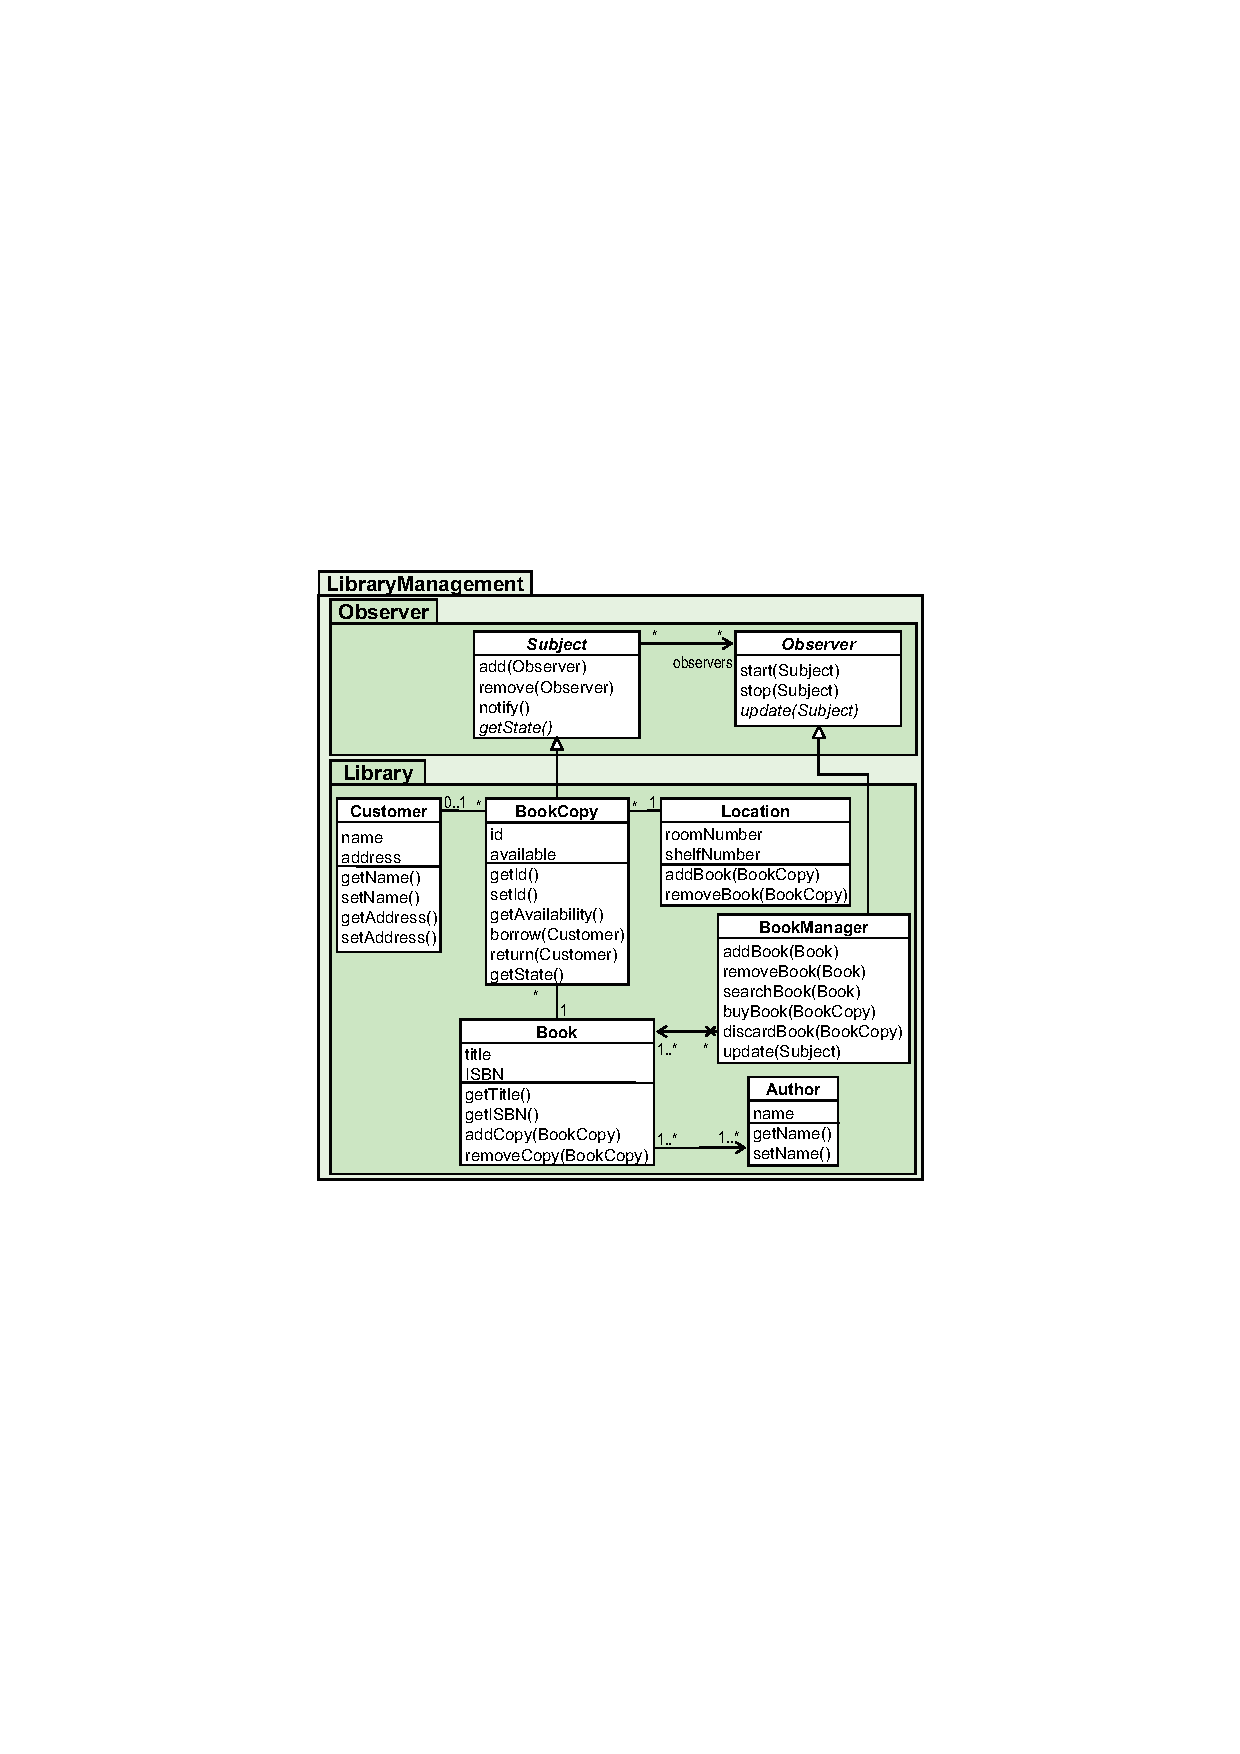
\includegraphics[width=0.7\textwidth]{figures/figure1}
	\caption{Sample figure}
	\label{fig:samplefigure_pdf}
\end{figure}


\section{Fonts}

When introducing important terms for the first time use \emph{emphasize}. For a consistent look and feel of proper names like {\cd} and {\uml{Observer}} pattern you may define macros in the main document \texttt{thesis.tex}.

\section{Code}

For short code fragments use the \textit{verbatim} environment.

\begin{verbatim}
//Start Program
System.out.println("Hello World!");
//End Program
\end{verbatim}

A much better alternative is the \textit{algorithm} environment (cf. Algorithm~\ref{alg:samplealgorithm}). This environment offers special formatting features for loops, operations and comments.

\begin{algorithm}[t]
\SetKwData{Left}{left}
\SetKwData{This}{this}
\SetKwData{Up}{up}
\SetKwFunction{Union}{Union}
\SetKwFunction{FindCompress}{FindCompress}
\SetKwInOut{Input}{input}
\SetKwInOut{Output}{output}

\Input{A bitmap $Im$ of size $w\times l$}
\Output{A partition of the bitmap}

\BlankLine

\emph{special treatment of the first line}\;
\For{$i\leftarrow 2$ \KwTo $l$}{
\emph{special treatment of the first element of line $i$}\;
\For{$j\leftarrow 2$ \KwTo $w$}{\label{forins}
\Left$\leftarrow$ \FindCompress{$Im[i,j-1]$}\;
\Up$\leftarrow$ \FindCompress{$Im[i-1,]$}\;
\This$\leftarrow$ \FindCompress{$Im[i,j]$}\;
\If(\tcp*[r]{O(\Left,\This)==1}){\Left compatible with \This}{\label{lt}
\lIf{\Left $<$ \This}{\Union{\Left,\This}}\;
\lElse{\Union{\This,\Left}\;}
}
\If(\tcp*[r]{O(\Up,\This)==1}){\Up compatible with \This}{\label{ut}
\lIf{\Up $<$ \This}{\Union{\Up,\This}}\;
\tcp{\This is put under \Up to keep tree as flat as possible}\label{cmt}
\lElse{\Union{\This,\Up}}\tcp*[r]{\This linked to \Up}\label{lelse}
}
}
\lForEach{element $e$ of the line $i$}{\FindCompress{p}}
}
\caption{Sample algorithm}\label{alg:samplealgorithm}
\end{algorithm}



%%%%%%%%%%%%%%%%%%%%%%%%%%%%%%%%%%%%%%%%%
\chapter{Bibliographic Issues}
\label{ch:bibliographic}
%%%%%%%%%%%%%%%%%%%%%%%%%%%%%%%%%%%%%%%%%

\section{Literature Search}

Information on online libraries and literature search, e.g., interesting magazines, journals, conferences, and organizations may be found at \url{http://www.big.tuwien.ac.at/teaching/info.html}.

\section{BibTeX}

BibTeX should be used for referencing.

The LaTeX source document of this pdf document provides you with different samples for references to journals~\cite{jour:B2BServices}, conference papers~\cite{proc:TheWebMLApproach}, books~\cite{book:umlatwork}, book chapters~\cite{incoll:ErhardKonrad1992}, electronic standards~\cite{man:BPEL}, dissertations~\cite{phdthesis:manuelWimmer}, masters' theses~\cite{mast:AUMLProfile}, and web sites~\cite{misc:BIGWebsite}. The respective BibTeX entries may be found in the file \texttt{references.bib}. For administration of the BibTeX references we recommend \url{http://www.citeulike.org} or JabRef for offline administration, respectively.


%%%%%%%%%%%%%%%%%%%%%%%%%%%%%%%%%%%%%%%%%
%%% BACKMATTER %%%%%%%%%%%%%%%%%%%%%%%%%%
%%%%%%%%%%%%%%%%%%%%%%%%%%%%%%%%%%%%%%%%%

\appendix

\bibliographystyle{plain}
\bibliography{references}

\end{document}
